\section{The revised prototypes}
We inherited a set of PowerPoint slides from the last year's product owner group.
This was a large collection of 122 slides where each slide was simply a single picture with clickable areas for simple navigation, making it difficult to update them.
Some of these slides were also not visually acceptable, leading to us making the decision of redoing the prototypes.
As described in \autoref{technologies-and-tools}, Adobe XD was used to create a new design and allow for interaction in the design.
The most relevant updated prototypes will be compared to the previous versions in the following section.

\subsection{The overall week plan view}
The main changes made in the overall view of the week plan is just the design. 
The top bar was changed to include new icons, and the generic phone/tablet bar was added to let the user keep an overview of the status of their device.
We removed the large area reserved for the name of the week plan on the previous suggestions, to give more space for the week plan to be used. 
\begin{figure}[H]
    \begin{subfigure}{0.5\textwidth}
    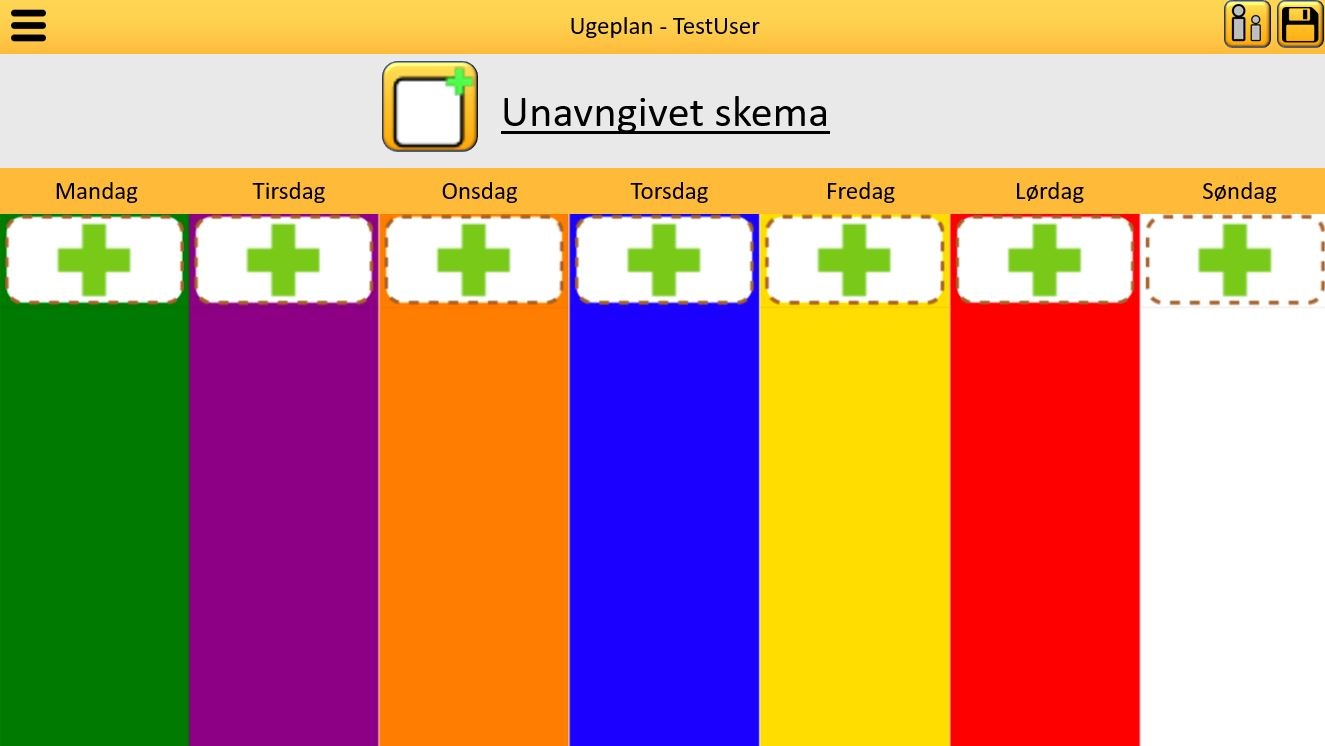
\includegraphics[width=1\linewidth, height=5cm]{previous_ugeplan.JPG} 
    \caption{The previous week plan view}
    \label{fig:previous_weekplan_view}
    \end{subfigure}
    \begin{subfigure}{0.5\textwidth}
        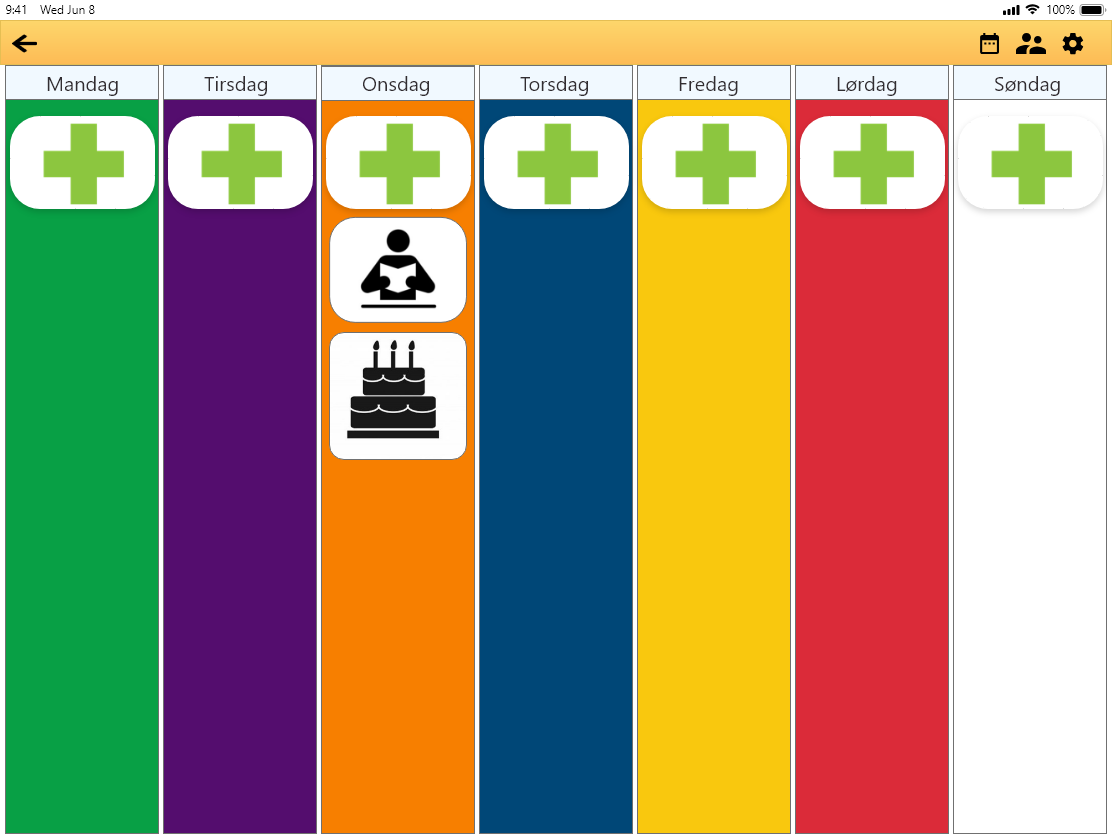
\includegraphics[width=1\linewidth, height=5cm]{ugeplan_citizen_view.png}
    \caption{The proposed new week plan view}
    \label{fig:new_weekplan_view}
    \end{subfigure} 
    \caption{This figure shows both designs for confirming password when changing from citizen to guardian.}
    \label{fig:weekplan_view}
\end{figure}

\subsection{The login screen and choosing citizen}
The base design of the previous login screen was functionally acceptable. 
The background colour used was just a dull yellow, and as such updated the background to be a little more dynamic but keeping the separate bars in which to input username and password.
The design change used for login in was also employed in the confirmation screen from swapping from citizen to guardian mode. 
The previous design and the new design for changing from citizen to guardian, as well as the general layout for logging in, can be viewed in the following figures:
\begin{figure}[H]
    \begin{subfigure}{0.5\textwidth}
    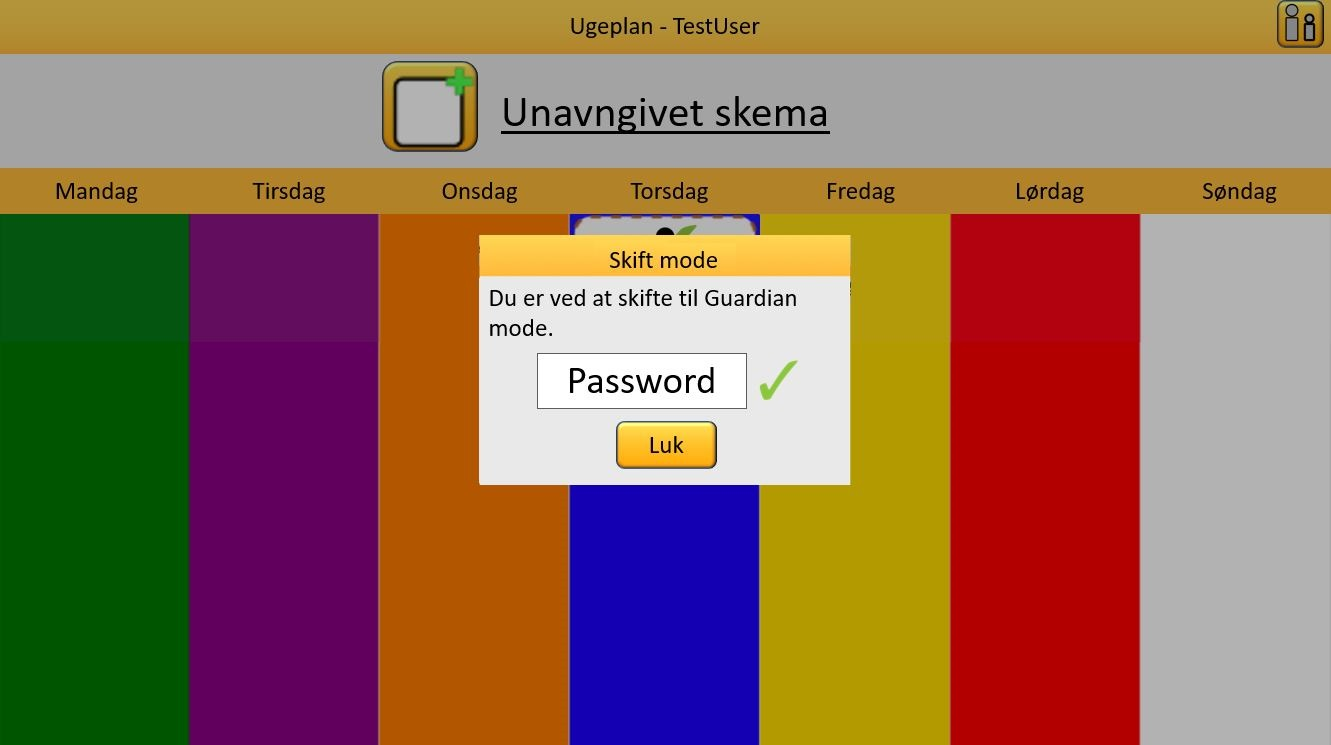
\includegraphics[width=1\linewidth, height=5cm]{previous_password_change.JPG} 
    \caption{The previous confirmation}
    \label{fig:previous_guardian_confirm}
    \end{subfigure}
    \begin{subfigure}{0.5\textwidth}
        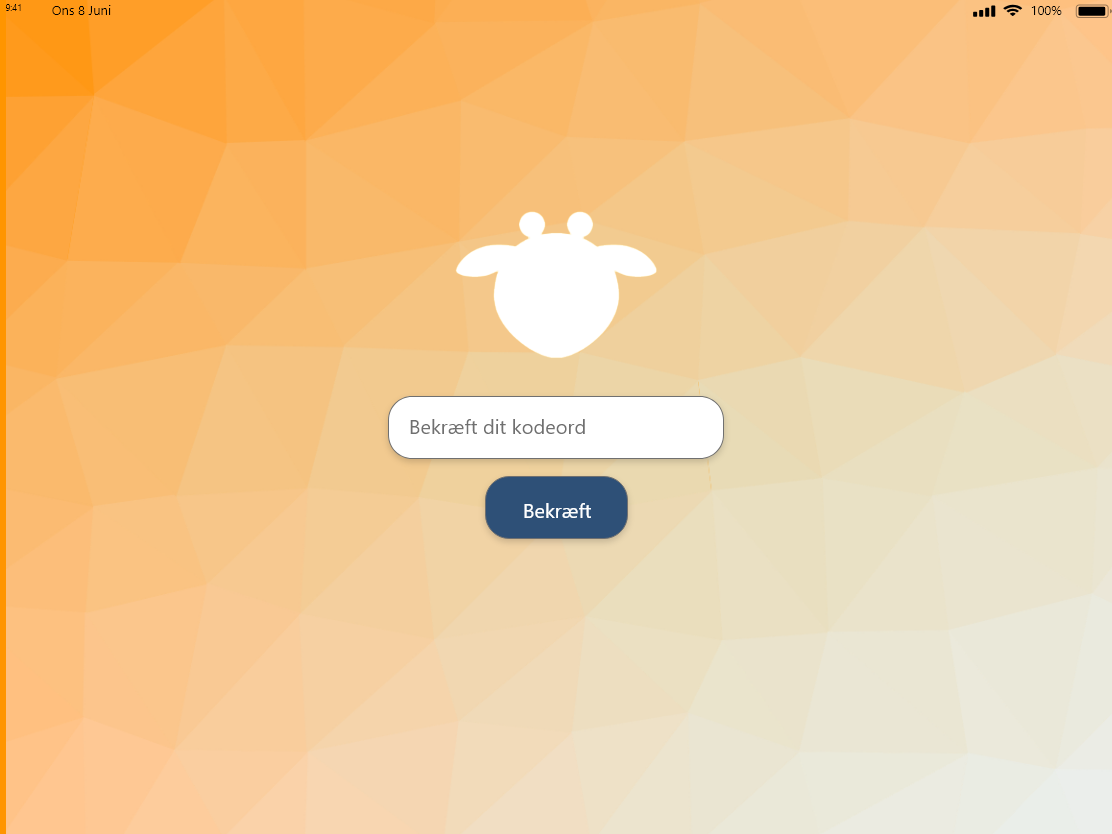
\includegraphics[width=1\linewidth, height=5cm]{guardian_switch_confirm.png}
    \caption{The proposed new change screen}
    \label{fig:new_guardian_confirm}
    \end{subfigure} 
    \caption{This figure shows both designs for confirming password when changing from citizen to guardian.}
    \label{fig:guardian_confirm}
\end{figure}
\noindent
The design of the page where citizens are selected was also changed.
It was  primarily changed to make it more aesthetically pleasing, with the main selection area being changed to a scrollable window with two columns. 
A comparison of the screen in which a citizen is selected is illustrated in the following figures:
\begin{figure}[H]
    \begin{subfigure}{0.5\textwidth}
    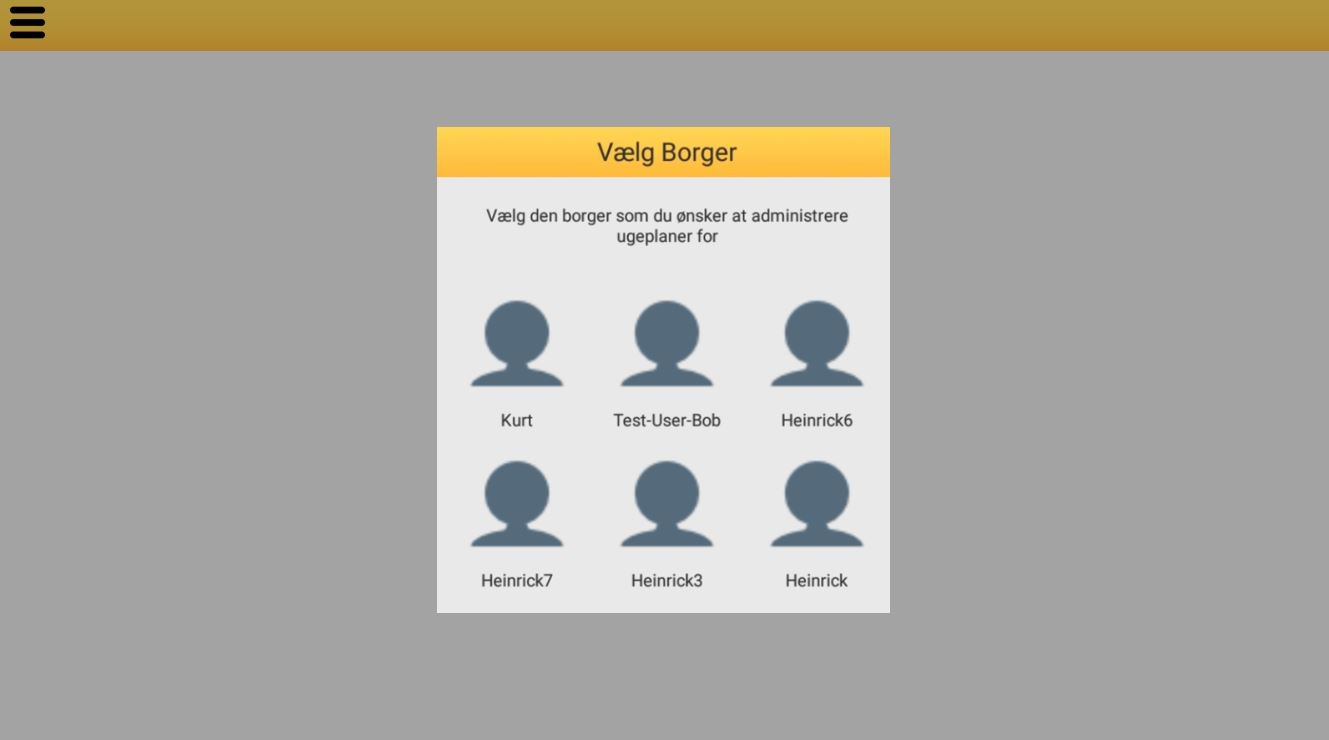
\includegraphics[width=1\linewidth, height=5cm]{previous_citizen_select.JPG} 
    \caption{The previous citizen selection}
    \label{fig:previous_guardian_confirm}
    \end{subfigure}
    \begin{subfigure}{0.5\textwidth}
        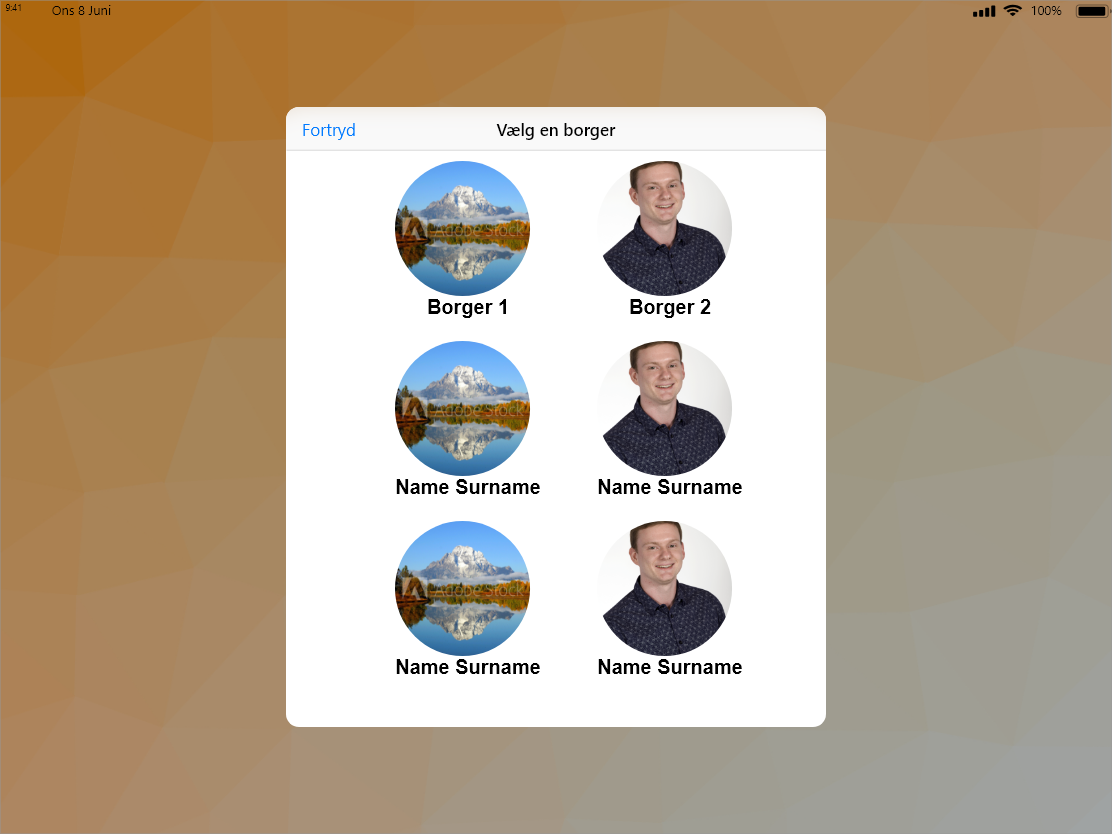
\includegraphics[width=1\linewidth, height=5cm]{copy_weekplan_choose_citizen.png}
    \caption{The proposed new citizen selection}
    \label{fig:new_guardian_confirm}
    \end{subfigure} 
    \caption{This figure shows both designs for choosing a citizen to view their week plans.}
    \label{fig:guardian_confirm}
\end{figure}
\noindent

\subsection{Greyscale functionality}
GIRAF should support the different preferences of the citizens. 
As such, a greyscale functionality is preferable.
This was also documented by the previous year, but they have not made a prototype for this functionality.
Instead, they proposed a yellow colour scheme.
We developed the greyscale prototype seen below with the intention to have it evaluated by company representatives.
\begin{figure}[H]
    \begin{subfigure}{0.5\textwidth}
    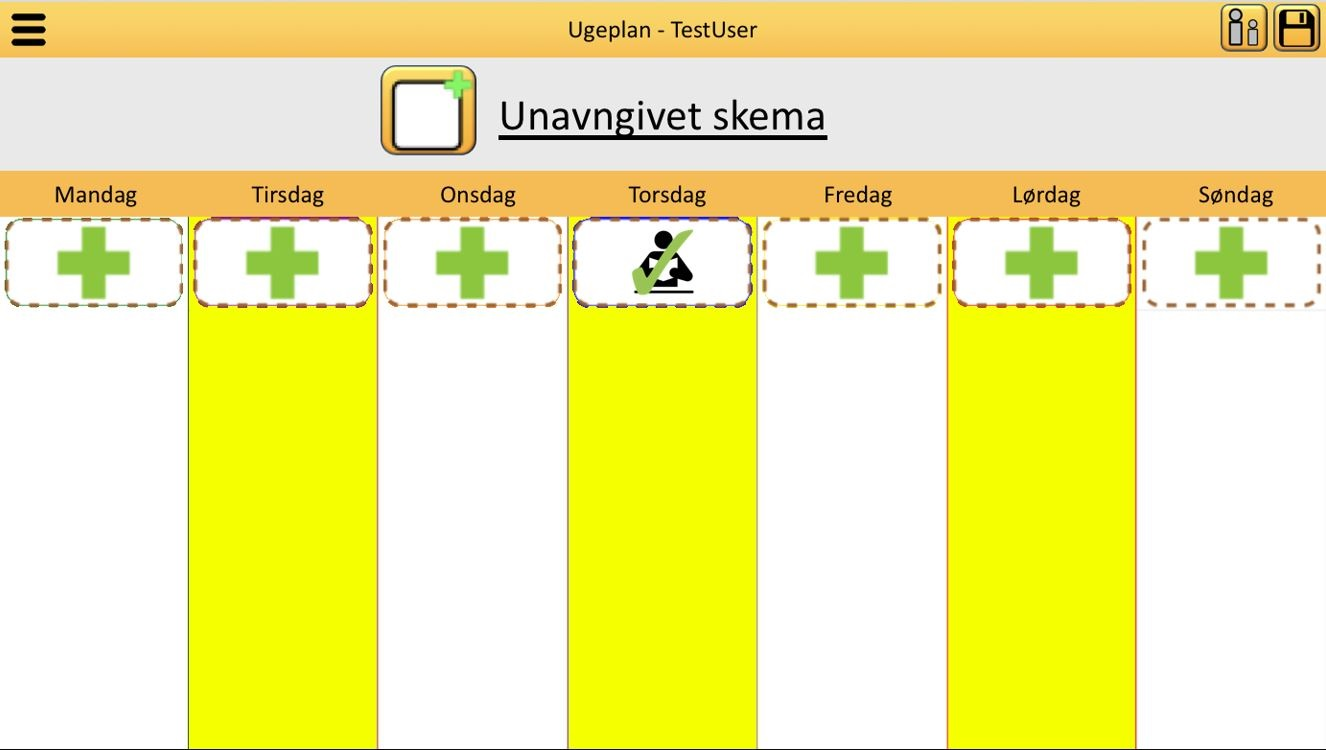
\includegraphics[width=1\linewidth, height=5cm]{previous_color_change.JPG} 
    \caption{The previous colour prototype}
    \label{fig:previous_citizen_select}
    \end{subfigure}
    \begin{subfigure}{0.5\textwidth}
        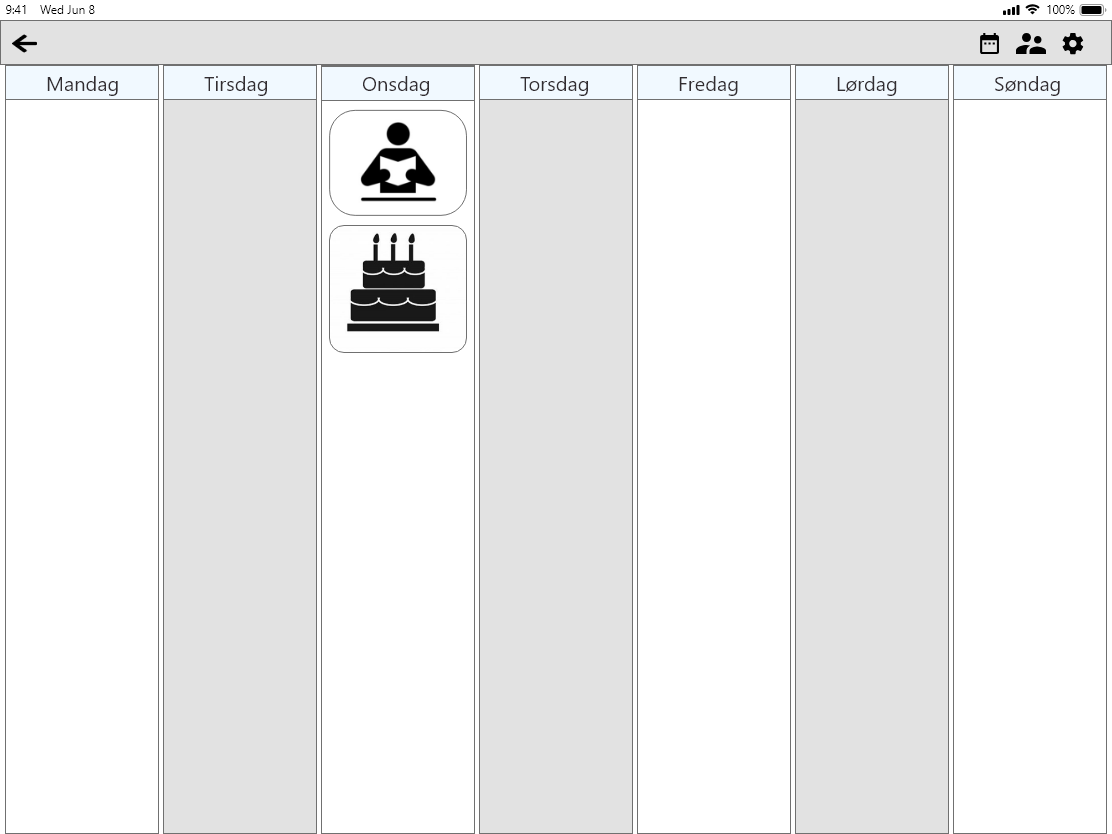
\includegraphics[width=1\linewidth, height=5cm]{greyscale_functionality.png}
    \caption{The proposed greyscale colouring}
    \label{fig:new_citizen_select}
    \end{subfigure} 
    \caption{This figure shows different colouring options.}
    \label{fig:citizen_select}
\end{figure}

